\chapter{Planung}
\label{cha:planung}

In diesem Kapitel werden Anforderungen an die Software und die Systemumgebung definiert sowie verwendete organisatorische Konzepte erläutert.

\section{Auswahl der Programmiersprache}

Die Software soll in der Skriptsprache Python entwickelt werden. Für die Entscheidung sprechen mehrere Vorteile: die Plattformunabhängigkeit wird durch die Verfügbarkeit von Interpretern sowohl für unix-artige Betriebssysteme als auch Windows ermöglicht. Die Software liegt jederzeit im Quellcode vor und kann so einfach gewartet und erweitert werden. Des Weiteren existiert aufgrund der hohen Popularität\footnote{\url{https://www.tiobe.com/tiobe-index/python/}} eine reichhaltige Auswahl an Bibliotheken und Onlinedokumentationen, welche die Entwicklung der Software vereinfachen. 

\section{Anforderungen}

Die Software soll auf den nicht-interaktiven Betrieb als Dienst auf unix-artigen Betriebssystemen ausgelegt werden. Dies hat u.\,a. Auswirkungen auf die geplanten Benutzerschnittstellen. Das Programm soll zur Laufzeit keine Konsoleneingaben verlangen, da diese nur bei einem interaktiven Betrieb, z.B. in der Shell, vorgenommen werden können. Stattdessen soll mit dem Anwender vollständig über den Telegram-Messenger interagiert werden und administrative Einstellungen sollen über Konfigurationsdateien vorgenommen werden können. 

Zur Anwendung von geänderten Einstellungen ist unter Umständen ein Neustart der Software notwendig. Die Software sollte daher zustandslos arbeiten, um einen möglichen Verlust von eingegangenen und noch nicht verarbeiteten Daten zu verhindern. Weiterhin sollte die durch einen Neustart verursachte Ausfallzeit so gering wie möglich gehalten werden. 

Die Software soll Ereignismeldungen über die Standardausgabe sowie über eine textbasierte Protokolldatei ausgeben, um Fehleranalysen zu vereinfachen. Es soll möglich sein, den Bot von mehreren Geräten gleichzeitig zu kontaktieren. Der Bot muss die Autorisierung von Benutzern prüfen, damit unerwünschter Datenabfluss verhindert wird.

\subsection{Systemumgebung}
Für den Betrieb der Software ist eine vorinstallierte Python 3 Umgebung notwendig. Zum Zeitpunkt der Entwicklung wurde die Version 3.9 verwendet. Die benötigten Bibliotheken sollen über den Paketmanager Pip bezogen und aktuell gehalten werden können. Auch wenn die Software auf den Betrieb als Dienst ausgelegt wird, soll eine interaktive Verwendung mit unix-artigen Betriebssystemen möglich sein. Außerdem ist eine Internetverbindung notwendig, um die Server der HTTP-APIs von Telegram und AWS zu erreichen. Graylog Open muss bereits installiert und an die zu überwachenden Systeme angeschlossen sein. Die Systemanforderungen entsprechen denen des verwendeten Betriebssystems. Da sämtliche Verbindungen zu externen Systemen via HTTP(S)-Verbindungen hergestellt werden, gibt es keine weiteren Anforderungen für den Betrieb der Software. Für eine Minimalkonfiguration kann die Software in vollem Funktionsumfang bereits beim Betrieb in einer Softwareentwicklungsumgebung, z.B. auf einem Notebook verwendet werden. Für den späteren Produktivbetrieb eignet sich ein System, welches günstig dauerhaft betrieben werden kann, beispielsweise eine AWS EC2-Instanz.

\section{Programmablauf}

\subsection{Selbsttest}
\label{sec:grundsaetzlicher-aufbau}

Nach dem Start der Software muss geprüft werden, ob ein einwandfreier Betrieb möglich ist. Dazu ist es notwendig, die Erreichbarkeit und Funktion sämtlicher Dienste mittels geeigneter API-Abfragen zu prüfen. Nachdem die Vorbereitungen abgeschlossen sind, kann in den Regelbetrieb übergegangen werden, in welchem sich das Programm bis zum Programmende befindet. 

\subsection{Regelbetrieb}

Im Regelbetrieb reagiert die Software in Echtzeit auf eingehende Nachrichten vom Anwender. 
Um den Betrieb der Software auch mit nicht-öffentlichen IP-Adressen (beispielsweise in einem Heimnetzwerk hinter einem NAT-Router) oder einer Firewall, welche den Zugriff auf Geräte im internen Netzwerk aus dem Internet verbietet, zu ermöglichen, soll das Verfahren des Long-polling für den Abruf von Informationen von der Telegram API verwendet werden (vgl. \hyperref[sec:telegram-getting-updates]{erstes Unterkapitel von Abschnitt 2.2.1}). Somit werden lediglich Verbindungen aus dem internen Netzwerk ins Internet aufgebaut. Eventuelle NAT-Router oder Firewalls hinterlegen den Verbindungsaufbau in internen Datenstrukturen wie NAT-Tabellen und lassen Antworten aus dem Internet zu.

Der geplante Ablauf des Regelbetriebs ist im Sequenzdiagramm in \autoref{fig:dia-seq} abgebildet.

\subsection{Spracherkennung}
\label{sec:spracherkennung}

Bei der Ausarbeitung eines Konzepts für die Funktionsweise der Spracherkennung müssen einige funktionale und nicht-funktionale Eigenschaften beachtet werden. Die Entscheidung wird u.\,a. beeinflusst durch Aspekte der ... 

\enlargethispage{0.5cm} 

\begin{itemize}
\item Erweiterbarkeit: es soll einfach und insbesondere ohne ein notwendiges Training von Sprachmodellen möglich sein, neue Systeme und Abfragen zu definieren.
\item Fehlertoleranz: die Aussprache einzelner Wörter verändert sich durch grammatikalische Eigenschaften je nach Satzbau leicht. Die Erkennung muss trotz dieser Veränderungen zuverlässig funktionieren.
\item Rechenkapazität: die Geschwindigkeit (Wartezeit während des Vorgangs) der Spracherkennung sollte nicht von begrenzten Rechenressourcen oder der Länge der zu übersetzenden Nachricht abhängen.
\item finanziellen Kosten: diese sollten möglichst gering gehalten werden.
\item Plattformunabhängigkeit: die Software und ggf. trainierte Modelle sollten wie die gewählte Programmiersprache Python plattformunabhängig und portabel sein.
\item Nachvollziehbarkeit: während der Entwicklung und bei der Bedienung sollten auftretende Fehler einfach erkenn- und behebbar sein.
\item Sprache: das System soll Sätze verstehen, welche Begriffe aus mehreren Sprachen (Deutsch und Englisch) beinhalten.
\end{itemize}

Es bestehen verschiedene Möglichkeiten, Sprache zu Text zu transkribieren und den Inhalt im Anschluss zu analysieren, um das Anliegen des Anwenders zu erkennen und eine passende Anfrage für die Suchmaschine in Graylog zu bilden. Für die Transkription ist es notwendig, künstliche Intelligenz einzusetzen. Diese kann lokal oder entfernt ausgeführt werden. Die entfernte Ausführung bietet Vorteile bezüglich der Plattformunabhängigkeit und der (von den lokalen Ressourcen unabhängigen) Geschwindigkeit. Es stehen verschiedene Online-Dienste für die Transkription zur Verfügung, darunter Watson Speech to Text von IBM, Amazon Transcribe von AWS und Speech-To-Text vom Anbieter Google Cloud. 

\subsubsection{Syntax}
\label{sec:syntax}

Liegt die eingegangene Nachricht als Text vor, müssen die Inhalte analysiert werden. Der Aufbau der Nachricht muss einem festen Muster folgen, welches durch eine Prozedur analysiert werden kann. Hierzu eignet sich die Verwendung von Schlüsselwörtern. Diese bieten den Vorteil, dass keine Analyse der Grammatik notwendig ist. Die Verwendung von künstlicher Intelligenz bietet hierbei keine Vorteile. Das KI-Modell müsste für neue Begriffsdefinitionen, Grammatik (Satzbau) sowie Umgangssprache trainiert werden. Dies ist bei der geplanten Anwendung des Programms nicht durchführbar, da der Aufwand für das Hinzufügen neuer Suchbegriffe möglichst gering gehalten werden soll. Weiterhin bietet ein Algorithmus für die Analyse einer Nachricht mit statischem Aufbau den Vorteil der besseren Nachvollziehbarkeit des ermittelten Ergebnisses.

Es wird ein Aufbau aus Produktkategorie, Eigenschaft und Zeitraum gewählt. Die Produktkategorie entspricht der abzufragenden Gerätegruppe, beispielsweise 'Webserver'. Für jede Produktkategorie können Eigenschaften definiert werden, für die Abfrage von Ereignissen mit einem Statuscode \lstinline{4xx} oder \lstinline{5xx} der Gruppe 'Webserver' beispielsweise 'Fehlermeldungen'. Ein weiteres Schlüsselwort führt zu den Informationen für den abzufragenden Zeitraum, welcher relativ angegeben wird ('letzte fünf Tage', 'letzte Woche', 'letzte 20 Minuten').

 \enlargethispage{0.5cm} 

\subsubsection{Vergleich diverser Transkriptionsdienste}
\label{sec:vergleich-transkrip}

Die Umwandlungsgenauigkeit der in \autoref{sec:spracherkennung} genannten Dienste soll mit einem Testset bestehend aus umzuwandelnden Audiodateien mit möglichen Sprachanfragen geprüft werden. Dazu wurden zehn Sprachnachrichten über die Telegram App für iOS auf einem iPhone aufgenommen. Im Anschluss wurden die Audiodaten von der Telegram API extrahiert, sodass diese im OGG-Format vorlagen. Die drei Dienste bevorzugen jeweils andere Audioformate, daher wurden die Dateien aus dem OGG-Format (für das Produkt von Google Cloud) in das MP3- (für das Produkt von AWS) und das FLAC-Format (für das Produkt von IBM) umgewandelt. Schließlich wurden jeweils zehn Audiodateien über eine Webkonsole, welche von allen Anbietern angeboten wurde\footnote{\url{https://eu-central-1.console.aws.amazon.com/transcribe/home?region=eu-central-1\#createJob}, \url{https://speech-to-text-demo.ng.bluemix.net}, \url{https://cloud.google.com/speech-to-text}}, an den Dienst übermittelt. Die Webkonsolen verwendeten jeweils die APIs, welche ebenfalls für den programmgesteuerten Zugriff verwendet werden. Die Ergebnisse werden in der \autoref{tab:erg-transkript} abgebildet.

\begin{figure}[h!]
\centering
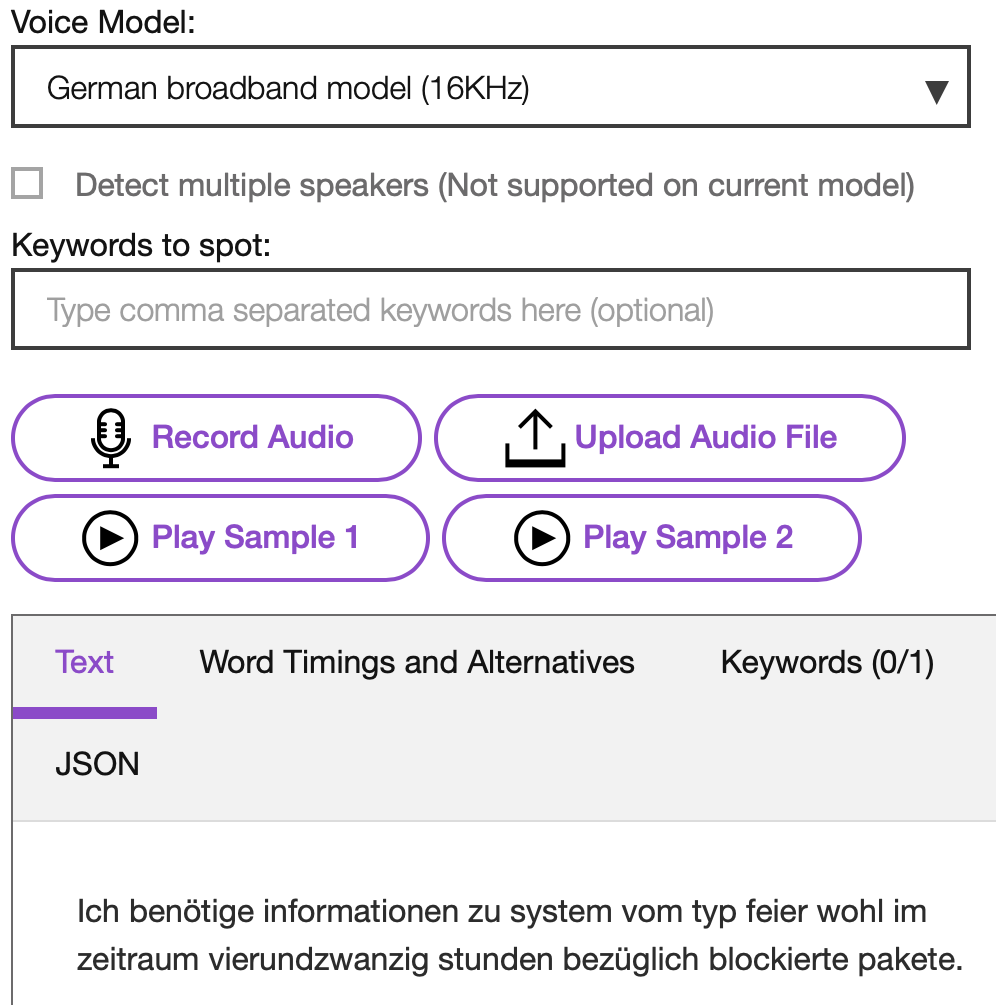
\includegraphics[scale=0.5]{feier-wohl}
\caption{Eingabemaske von IBM Watson Speech to Text nach Bearbeitung von Testset06 mit einer unzutreffenden Ausgabe.}
\label{fig:feier-wohl}
\end{figure}

Die Audionachrichten beinhalten folgende gesprochene Texte:
\begin{itemize}
\item \textit{Testset01}: "Typ Webserver Eigenschaft Fehler Zeitraum 24 Stunden"
\item \textit{Testset02}: "Typ Webserver bezüglich Erreichbarkeit Zeitraum 24 Stunden"
\item \textit{Testset03}: "Typ Webserver bezüglich Besucherzugriffe Zeitraum 24 Stunden"
\item \textit{Testset04}: "Typ Webserver bezüglich Besucherzugriffe Zeitraum 24 Stunden"
\item \textit{Testset05}: "Ich benötige Informationen zu Systemen vom Typ Firewall im Zeitraum 24 Stunden bezüglich blockierte Pakete"
\item \textit{Testset06}: "Typ eins bezüglich drei Zeitraum ein Tag"
\item \textit{Testset07}: "Typ eins bezüglich drei Zeitraum ein Tag"
\item \textit{Testset08}: "Typ Webserver Zeitraum 24 Stunden bezüglich Erreichbarkeit"
\item \textit{Testset09}: "Typ Webserver Zeitraum 24 Stunden bezüglich Erreichbarkeit"
\item \textit{Testset10}: "Typ Mailserver bezüglich empfangene Mails Zeitraum ein Jahr"
\end{itemize}

\begin{table}[hb!]
\centering
\begin{tabular}{c|c|c|c}
Testset 		& AWS	& Google		& IBM \\
\hline
01			& -		& +			& + \\
02			& +		& +			& - \\
03			& +		& +			& + \\
04			& -		& -			& - \\
05			& +		& +			& - \\
06			& +		& +			& - \\
07			& +		& +			& - \\
08			& +		& +			& - \\
09			& +		& -			& - \\
10			& +		& +			& - \\
\hline
Summe Fehler	& 2		& 2			& 8
\end{tabular}
\caption{Ergebnisse der Transkriptionsaufträge.}
\label{tab:erg-transkript}
\end{table}

Die Transkriptionsdienste von AWS und Google Cloud konnten durch eine geringe Fehlerquote gegenüber dem Produkt vom IBM überzeugen. Aufgrund von bereits existierenden persönlichen Erfahrungen in der Verwendung von AWS wird Amazon Transcribe als Transkriptionsdienst verwendet.

\subsubsection{Konfiguration des Bots}

Die Erweiterung der Software soll einfach möglich sein. Produktgruppen sollten darüber hinaus dynamisch erweiterbar sein: Wird eine Abfrage für die Produktkategorie 'Webserver' getätigt, sollen alle derzeit an Graylog angeschlossenen Webserver in die Suche einbezogen werden. 

Die Software ist für die Bedienung durch Systemadministratoren vorgesehen. Daher soll für die Konfiguration der Abfragen eine Textdatei verwendet werden. Diese ermöglicht eine schnelle Anpassung der Konfiguration und bietet gleichzeitig einen Überblick über bestehende Suchbegriffe. Für die einfache Verwendung mit einer Python-Bibliothek stehen mehrere Dateiformate zur Verfügung, darunter JSON, INI, TOML, YAML und XML. Das YAML- und XML-Format ist für die Verwaltung über einen Texteditor ohne Syntaxhervorhebung und Funktionen wie automatischem Einrücken nicht geeignet. 

Das TOML-Format vereint die Vorteile der einfachen Lesbarkeit des INI-Formats mit den Vorteilen der Verwendung von verschiedenen Datentypen des JSON-Formats. TOML entspricht weitestgehend der INI-Syntax. Ein Unterschied besteht darin, dass von der Spezifikation verschiedene Datentypen unterstützt werden\footnote{\url{https://toml.io/en/v1.0.0}}, darunter Zeichenketten (engl. Strings). Diese können im Falle von enthaltenen Leerzeichen in Anführungszeichen geschrieben werden. Die Hierarchie innerhalb einer TOML-Datei kann mit dem im \hyperref[sec:syntax]{vorherigen Unterkapitel "Syntax"} beschriebenen Aufbau abgebildet werden. TOML-Sektionen werden mit eckigen Klammern markiert und entsprechen den Produktkategorien (vgl. zweite Zeile des \autoref{toml-syntax}). Sie beinhalten Name-Wert-Paare, welche durch ein Gleichheitszeichen getrennt werden (vgl. dritte Zeile des \autoref{toml-syntax}). Ein Name darf in einer Sektion nur jeweils einmal vorkommen, eine Sektion darf in einer Datei nur jeweils einmal vorkommen. Sektionen, Name und Werte dürfen Leerzeichen enthalten. Name und Werte werden in diesem Fall in Anführungszeichen gesetzt und so als String definiert. Die im \hyperref[sec:syntax]{vorherigen Unterkapitel "Syntax"} definierten Eigenschaften von Produktkategorien werden durch die Namen in der TOML-Syntax repräsentiert. Die mit den Eigenschaften verknüpften Suchbegriffe werden durch die Werte der Name-Wert Paare in der TOML-Syntax repräsentiert. Zusätzlich ist es möglich, einzeilige Kommentare mit \lstinline{#} einzuleiten.

\begin{lstlisting}[caption={Beispiel der TOML-Syntax.}, label=toml-syntax, xleftmargin=6mm]
# Dies ist ein Kommentar
[Sektion]
Name = "Wert"

[Webserver]
Fehler = http_response_code:[400 TO 599] 
\end{lstlisting}

\begin{figure}[h!]
\centering
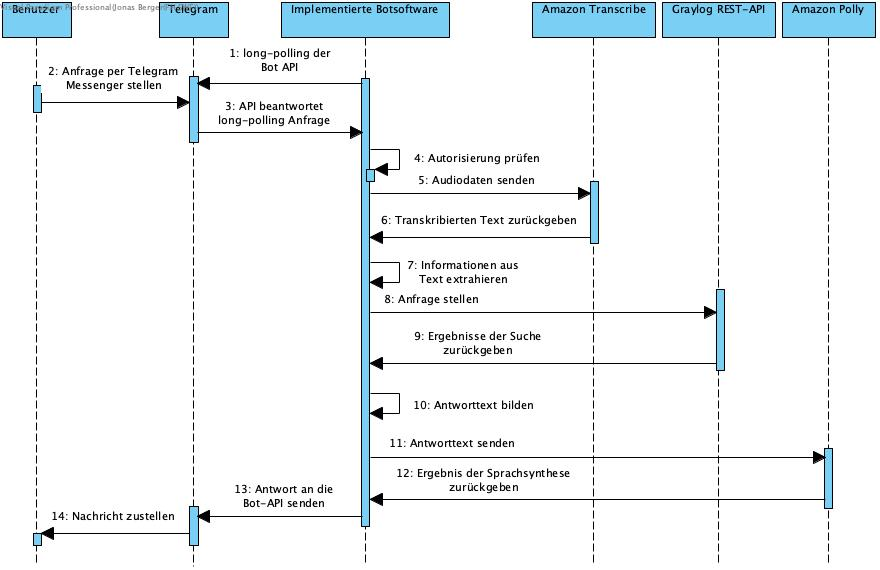
\includegraphics[scale=0.8,angle=90,origin=c]{dia-seq}
\caption{Sequenzdiagramm für Regelbetrieb.}
\label{fig:dia-seq}
\end{figure}
